\section{Glove Block Design}

The glove block will manage inputs from and outputs to the two gloves the player
wears while using the game. Two modules comprise the entire block.

\begin{figure}
\centering
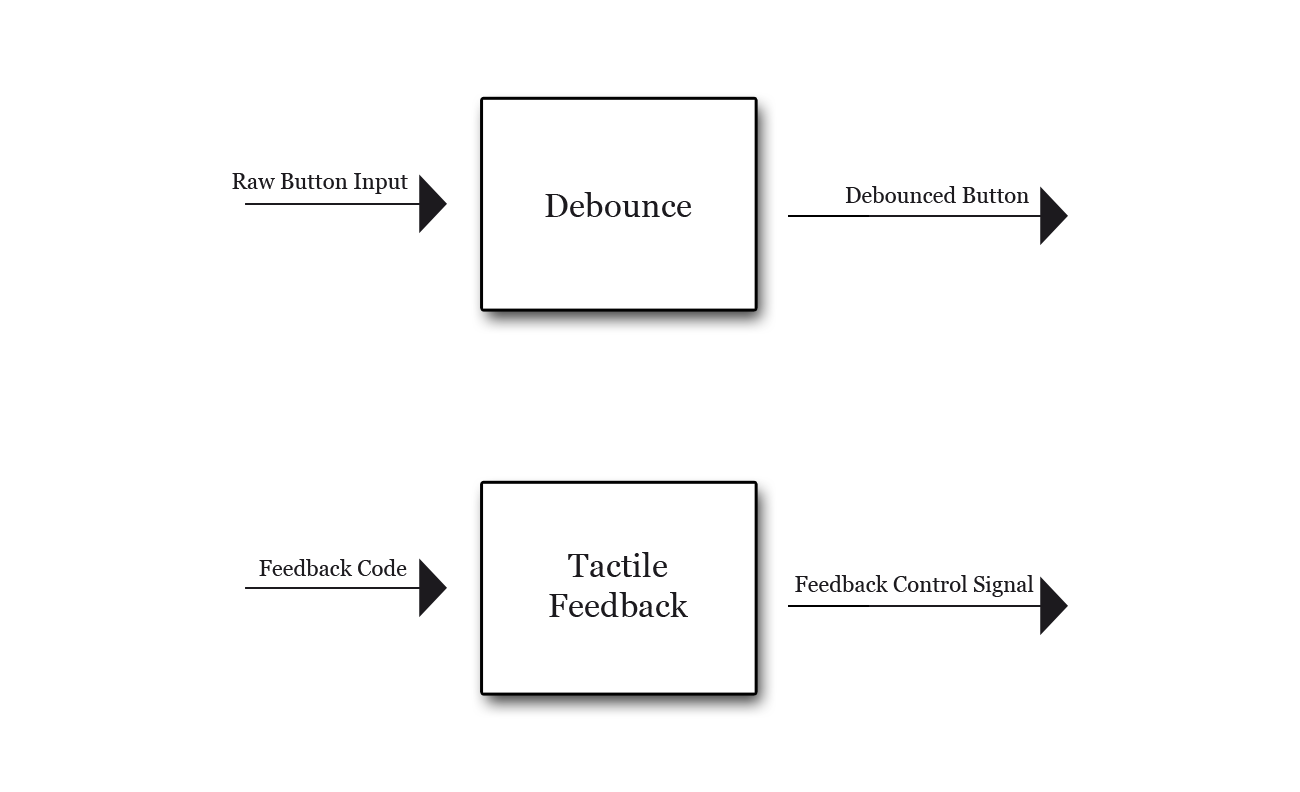
\includegraphics[scale=1]{img/glove.png}
\caption{The glove system is comprised of two data processing steps, one for the
debouncing of button input and the other for processing of tactile feedback duty
cycles.}
\label{fig:glove}
\end{figure}

\subsection{Tactile Feedback}

The tactile feedback module takes as input a short sequence of bits from the
gameplay block and outputs two signals to the gloves, one for each vibration
motor. The complexity of this system is minimal. It will use a divider and a
couple counting registers in order to control the duty cycles of the two motors.

A stretch goal would be do add additional vibration motors to provide more
complex tactile feedback. This would require a simple expansion of the inputs
and outputs of this module, allowing for the use of more complex information
about the placement of hands and objects on screen.

\subsection{Debounce}

The debounce module will take the raw output of two buttons from the gloves and
prevent dirty or asynchronous input. The 6.111-provided debounce module will be
used.
